
\documentclass[../../tex_main/NEMO_manual]{subfiles}

\begin{document}




% ================================================================
% Chapter 6 � Radiative transfer
% ================================================================

\chapter{Radiative transfer}
\label{chap:RAD}
\minitoc

\newpage
$\ $\newline    % force a new line

Radiative transfer in SI$^3$ currently reduces to the parameterization of solar radiation partitionning through the snow/ice/open water system, treated using a single wavelength band. This will likely be improved in future versions of the code. In this chapter, we first explain how solar radiation is partionned in the snow-ice system, then describe how, solar radiation-wise, the snow-ice system is framed in the context of the atmosphere-ice-ocean boundary.

\section{Solar radiation partitionning in the snow-ice system}

%--------------------------------------------------------------------------------------------------------------------
%
% FIG x : Radiation balance %
\begin{figure}[!ht]
\begin{center}
\vspace{0cm}
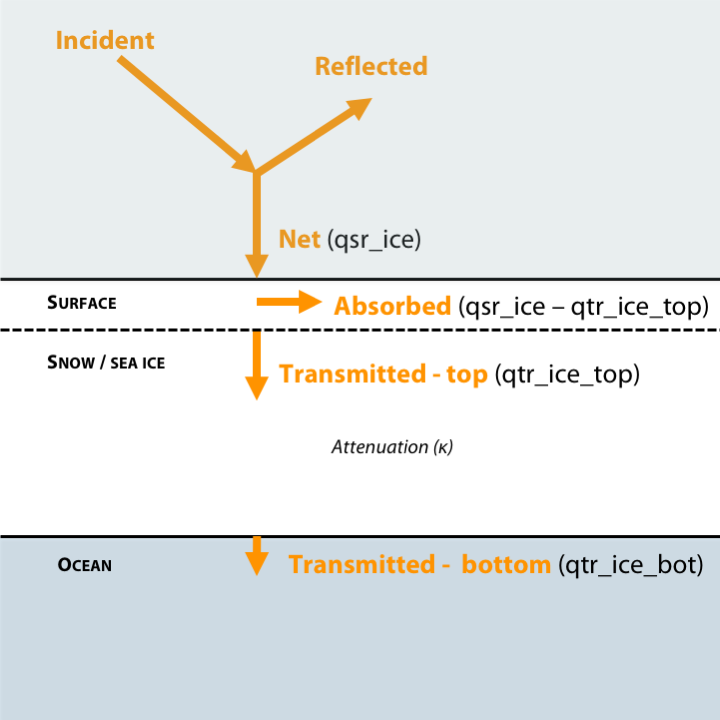
\includegraphics[height=6cm,angle=-00]{../Figures/radiative_transfer.png}
\caption{Partitionning of solar radiation in the snow-ice system, as represented in SI$^3$.}
\label{fig_radiative_transfer}
\end{center}
\end{figure}
%
%--------------------------------------------------------------------------------------------------------------------

Solar radiation in the snow-ice system is represented following the principles of \cite{MaykutUntersteiner71}, see Fig.\ref{fig_radiative_transfer}, using a unique band of solar radiation. Incident solar radiation (W/m$^2$, counted per unit ice area - not per grid cell area) is specified in the SBC routines and is a priori category dependent, because multiple atmosphere-surface reflexions are frequent in polar regions imply that incident radiation depends on the surface albedo and therefore surface state. 

Net solar radiation qsr\_ice(i,j,l) is obtained by substracting the reflected part of the incident radiation using the surface albedo $\alpha(i,j,l)$, parameterized as a function of environmental conditions. 

The subsequent attenuation of solar radiation through the snow-ice system is represented assuming the presence of a highly diffusive surface scattering layer, absorbing a fraction $i_o$ of net solar radiation, which is transformed into sensible heat, contributing to the surface energy balance. 

The remainder of solar radiation, qtr\_ice\_top(i,j,l), is transmitted below the surface and attenuates following Beer-Lambert law. The part of solar radiation that is absorbed on its path to the base of the ice is given as sensible heat to the snow/ice system, via a source term in the heat diffusion equation. The rest of solar radiation that reaches the ice base, qtr\_ice\_bot(i,j,l), is transmitted to the ocean. 

In the rest of this section, we describe how the albedo, the surface transmission parameter $i_o$ and the attenuation of solar radiation are parameterized.

\subsection{Surface albedo}

The surface albedo determines the amount of solar radiation that is reflected by the ice surface, hence also net solar radiation. The philosophy of the parameterization of surface albedo is the following: each ice category has its own albedo value $\alpha(i,j,l)$, determined as a function of cloud fraction, ice thickness, snow depth, melt pond fraction and depth, using observation-based empirical fits. 

The original \cite{ShineHenderson85} parameterization had a few inconsistencies and flaws that the revisited parameterization described hereafter fixes. In particular, the dependencies of albedos on ice thickness, snow depth and cloud fraction have been revised in the light of recent observational constraints \citep{Brandtetal05,GrenfellPerovich04}. In addition, the asymptotic properties of albedo are better specified and now fully consistent with oceanic values. Finally, the effect of melt ponds has been included \citep{Lecomteetal15}.

The user has control on 5 reference namelist values, which describe the asymptotic values of albedo of snow and ice for dry and wet conditions, as well as the deep ponded-ice albedo. Observational surveys, in particular during SHEBA in the Arctic \citep{Perovichetal02alb} and further additional experiments \citep{GrenfellPerovich04}, as well as by \cite{Brandtetal05} in the Antarctic, have provided relatively strong constraints on the surface albedo. In this context, the albedo can hardly be used as the main model tuning parameter, at least outside of these observation-based bounds (see namalb for reference values).

\forfile{../namelists/namalb}

%--------------------------------------------------------------------------------------------------------------------
%
% FIG x : cloud correction
%
\begin{figure}[ht]
\begin{center}
\vspace{0cm}
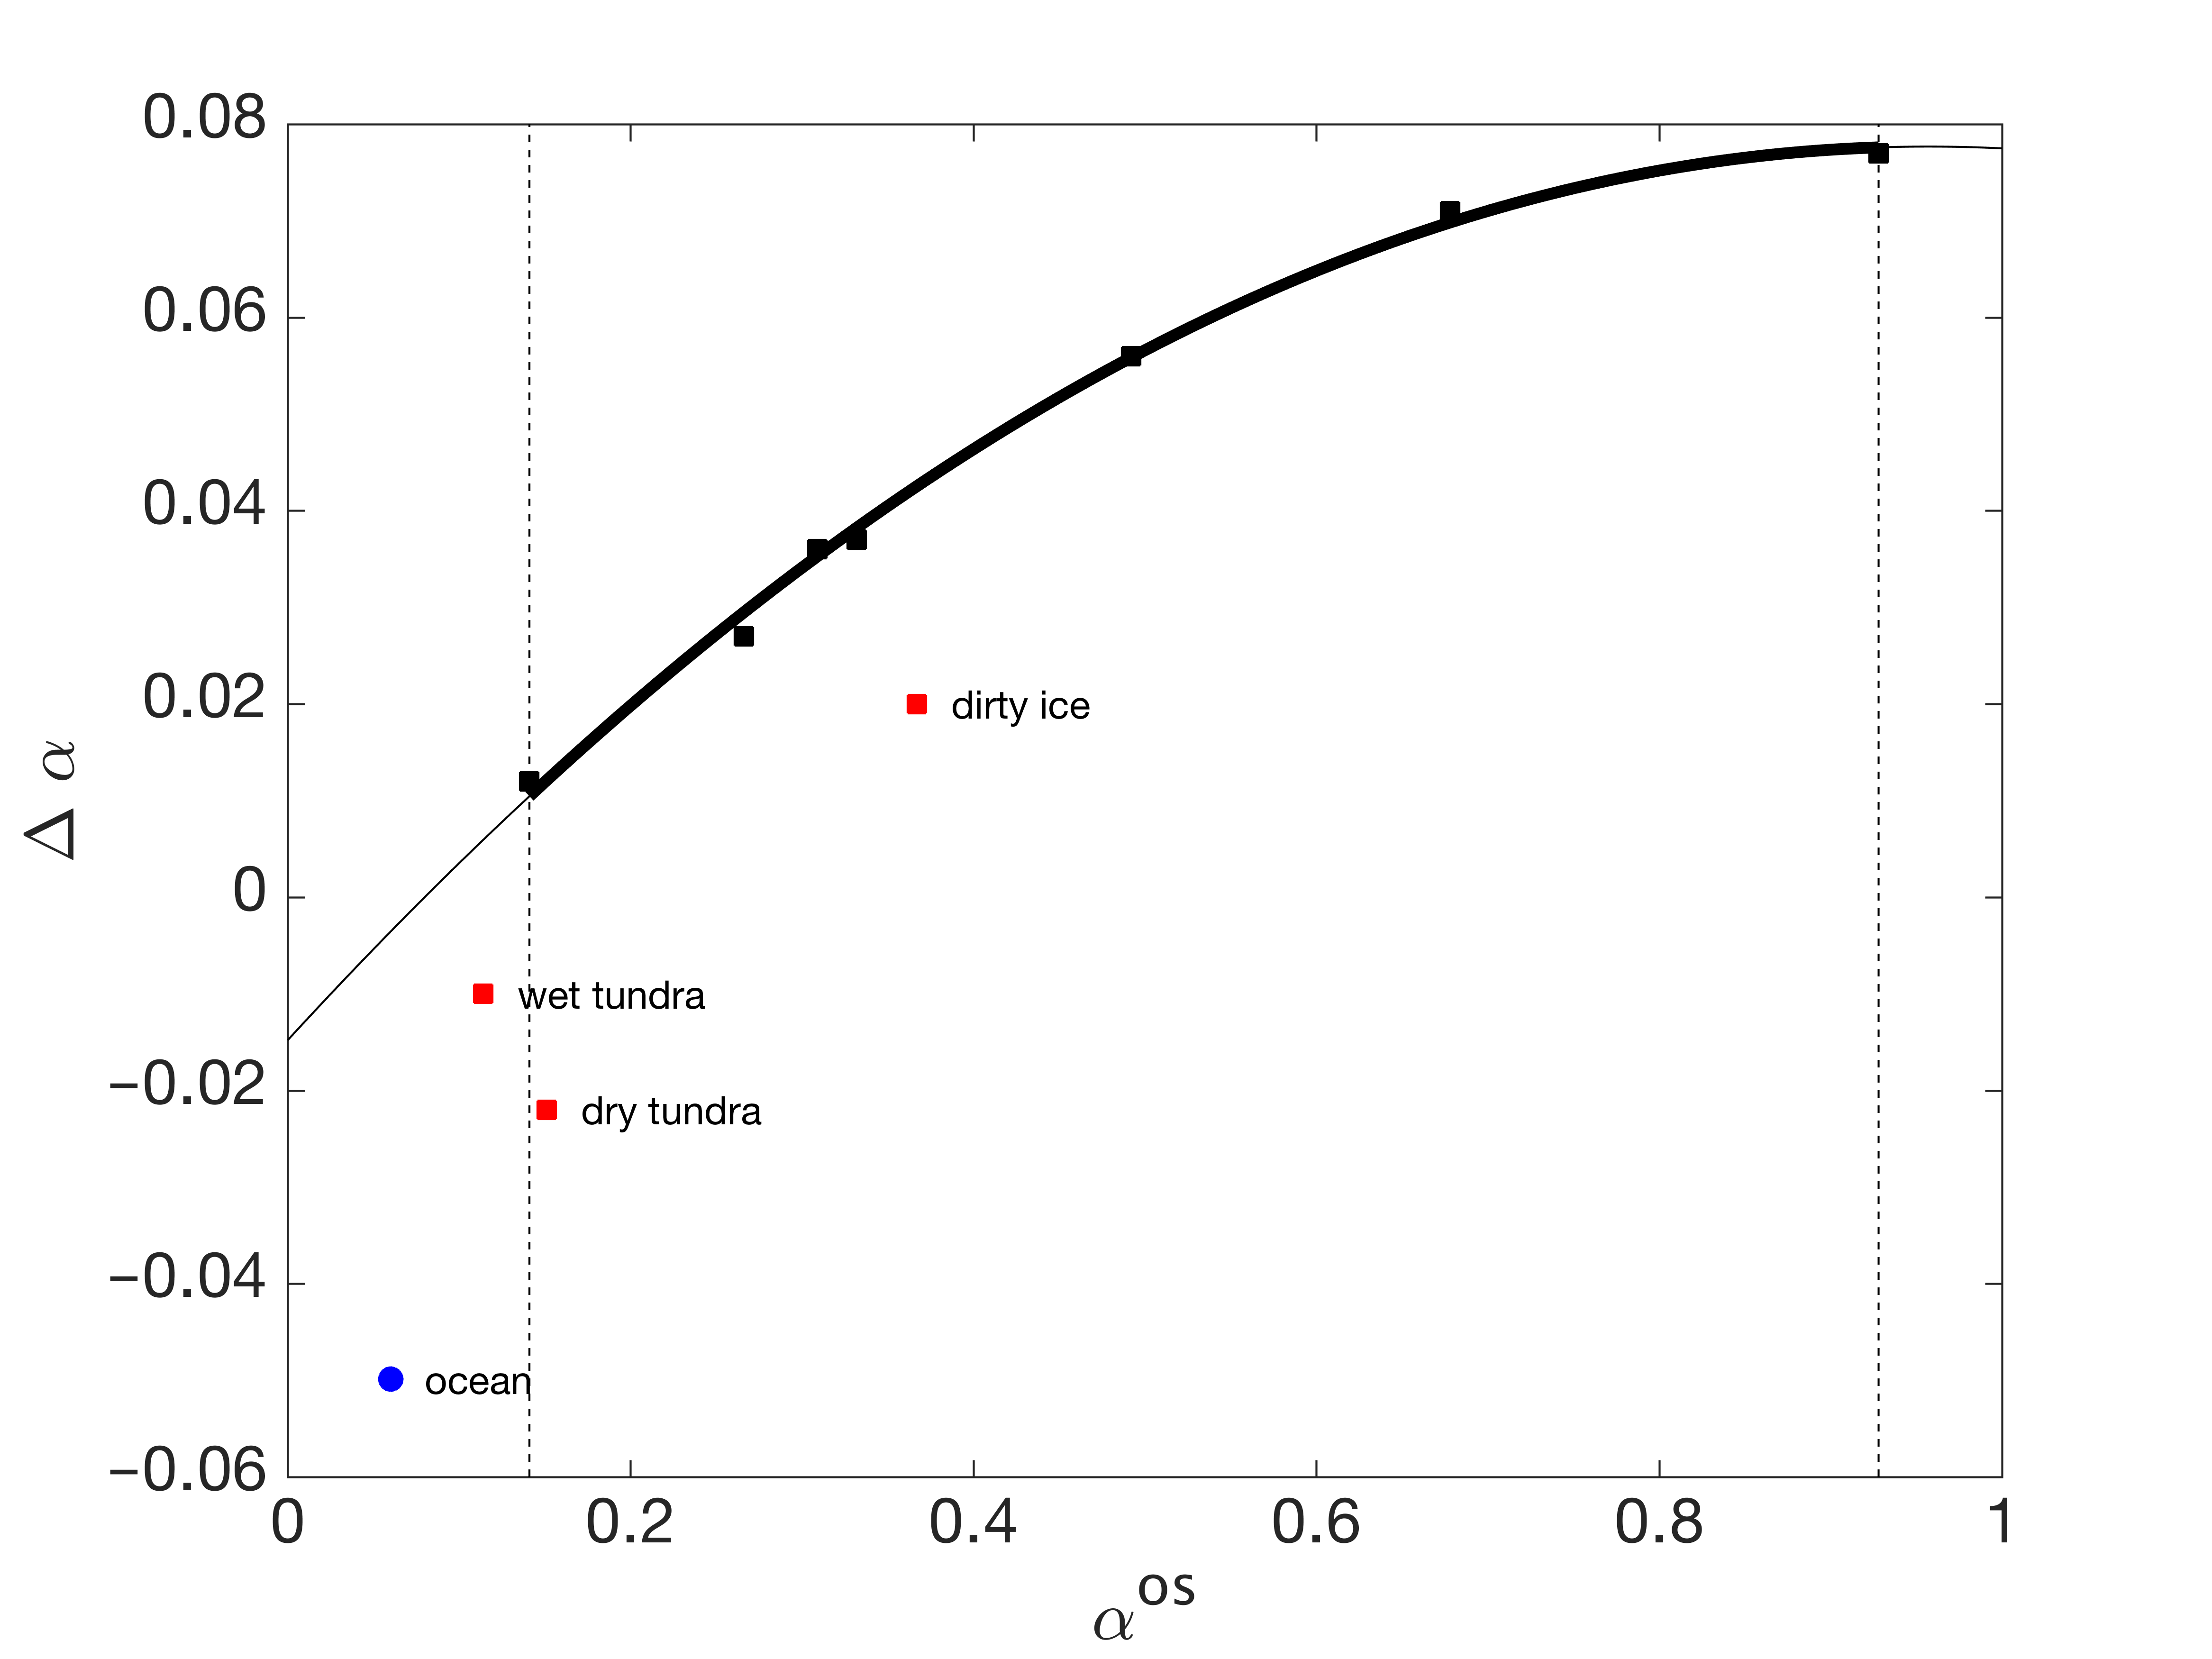
\includegraphics[height=10cm,angle=-00]{../Figures/albedo_cloud_correction.png}
\caption{Albedo correction $\Delta \alpha$ as a function of overcast sky (diffuse light) albedo $\alpha_os$, from field observations \cite[][their Table 3]{GrenfellPerovich04} (squares) and 2nd-order fit (Eq. \ref{eq_albedo_cloud_correction}). Red squares represent the irrelevant data points excluded from the fit. For indication, the amplitude of the correction used in the ocean component is also depicted (blue circle).}
% ocean uses 0.06 for overcast sky (Payne 74) and Briegleb and Ramanathan parameterization
\label{fig_albedo_cloud_correction}
\end{center}
\end{figure}
%
%--------------------------------------------------------------------------------------------------------------------

Because the albedo is not an intrinsic optical property, it depends on the type of light (diffuse of direct), which is practically handled by weighting the clear (cs) and overcast (os) skies values by cloud fraction $c(i,j)$ \citep{FichefetMaqueda97}:
\begin{equation}
\alpha(i,j,l) = [ 1 - c(i,j) ] \cdot \alpha_{cs} (i,j,l) + c (i,j) \cdot \alpha_{os}(i,j,l).
\end{equation}
For concision, we drop the spatial and category indices hereafter. \cite{GrenfellPerovich04} observations at Point Barrow, on the Alaskan Coast, suggest that clear and overcast sky albedos are directly related through
\begin{equation}
\alpha_{cs} = \alpha_{os} - \Delta \alpha(\alpha_{os}).
\end{equation}
The relation between $\Delta \alpha$ and $ \alpha_{os}$ can well be handled using a 2$^{nd}$-order polynomial fit (Fig. \ref{fig_albedo_cloud_correction}):
\begin{equation}
\Delta \alpha =  ( -0.1010 \cdot \alpha_{os}^2 + 0.1933 \cdot \alpha_{os} - 0.0148 ).
\label{eq_albedo_cloud_correction}
\end{equation}
Overcast sky surface albedo is used as a reference, from which the clear-sky value is derived.

%--------------------------------------------------------------------------------------------------------------------
%
% FIG x : thickness, snow depth, pond depth dependencies
%
\begin{figure}[ht]
\begin{center}
\vspace{0cm}
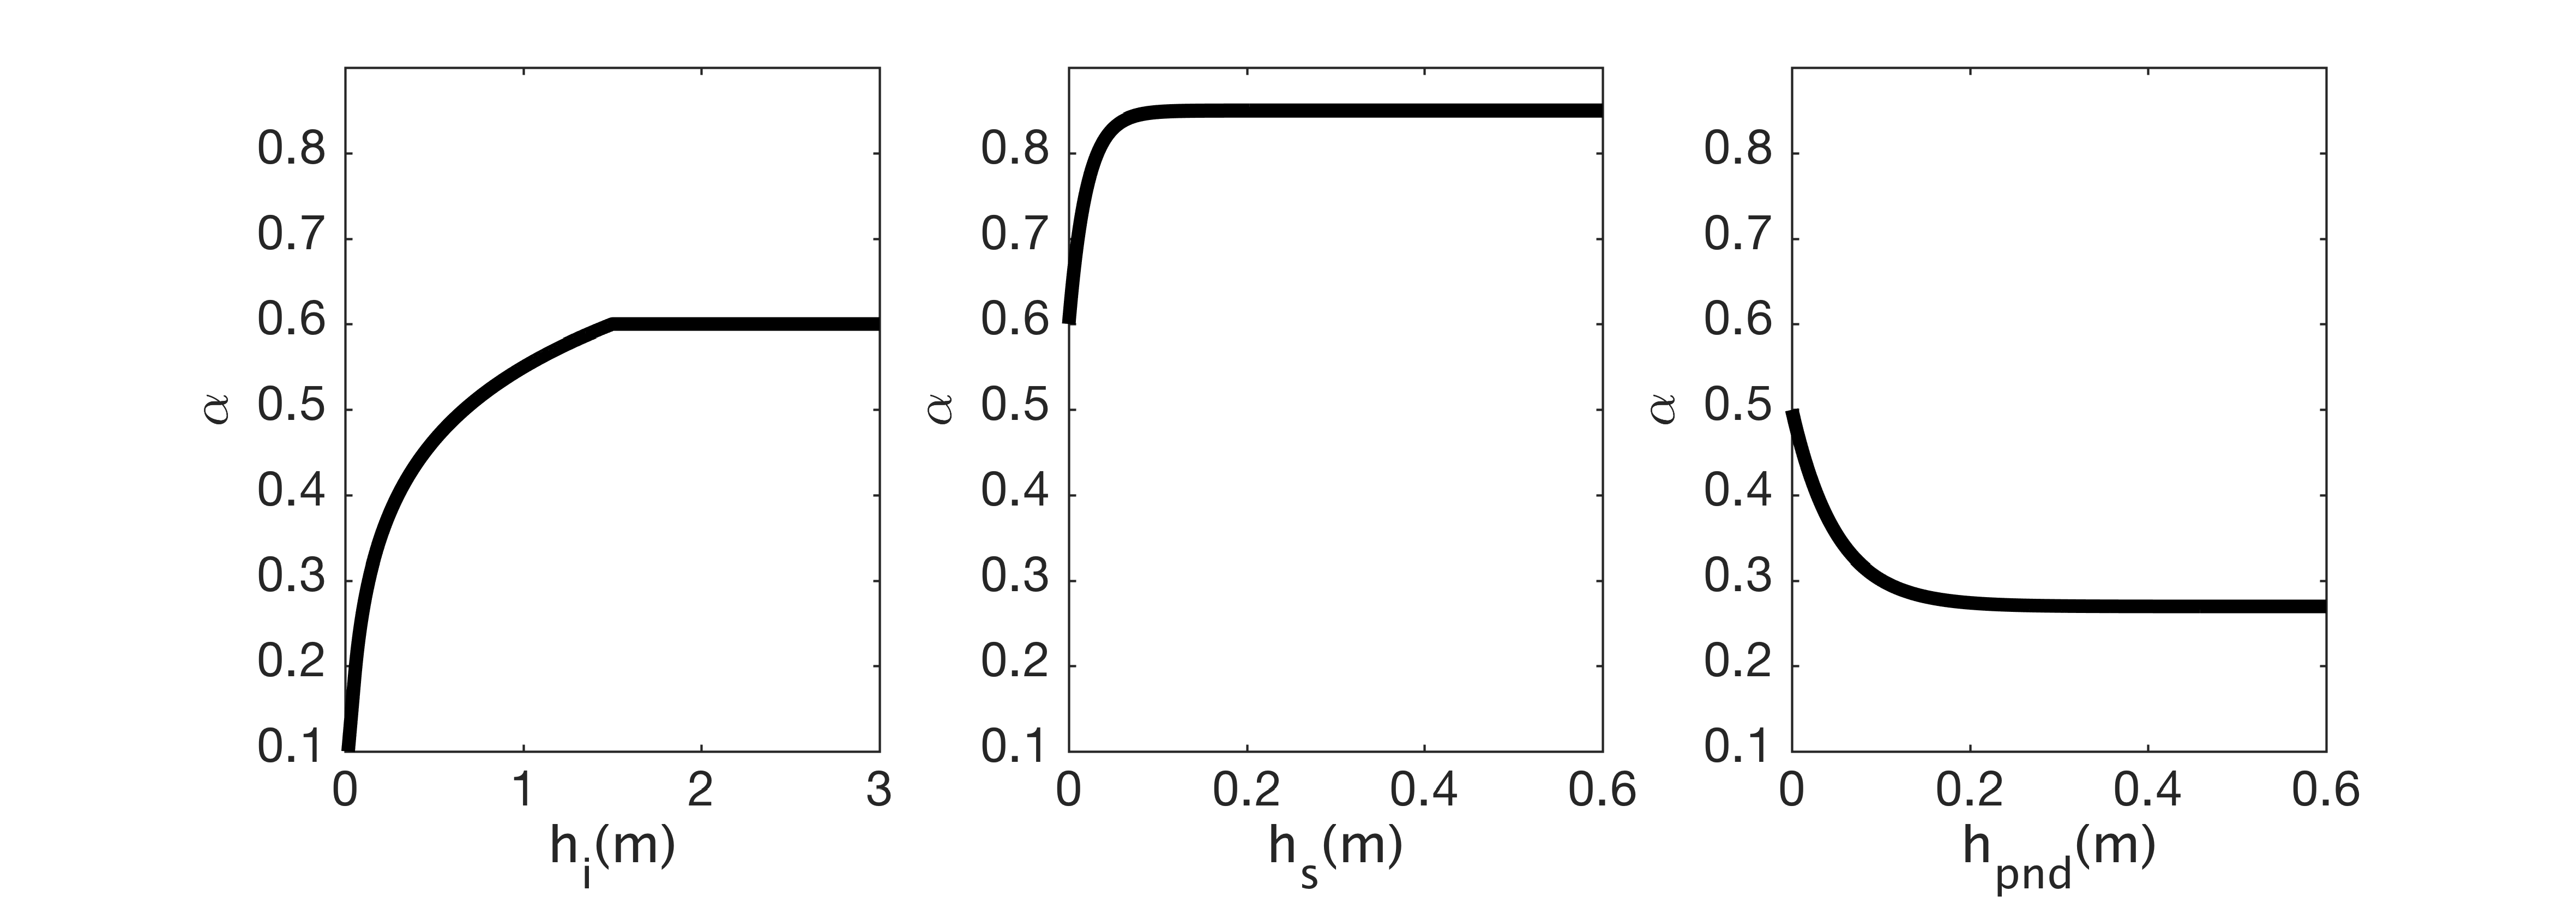
\includegraphics[height=4cm,angle=-00]{../Figures/albedo_dependencies.png}
\caption{Example albedo dependencies on ice thickness, snow depth and pond depth, as parameterized in SI$^3$.}
\label{fig_albedo_dependencies}
\end{center}
\end{figure}
%
%--------------------------------------------------------------------------------------------------------------------

The second important parameter that controls surface albedo is surface type. In each category, we assume that three types of surfaces can coexist (bare, snow-covered and ponded ice), with respective fractions $f_{ice}$, $f_{snw}$ and $f_{pnd}$ summing to 1. Then the overcast albedo is expressed as
\begin{equation}
\alpha_{os}(i,j,l) = f_{ice} \cdot \alpha_{ice} + f_{snw} \cdot \alpha_{snw} + f_{pnd}\cdot \alpha_{pnd}
\end{equation}
with a specific albedo value for each surface type. 

The surface fractions $f_{ice}$, $f_{snw}$ and $f_{pnd}$ are currently crudely parameterized: if snow is present ($h_s>0$), then $f_{snw}=1$ and $f_{ice}=f_{pnd}=0$. In the absence of snow, $f_{pnd}$ is either specified or calculated (depending on melt pond options in nampnd), and $f_{ice}=1.-f_{pnd}$. Admittedly, more refined parameterizations of $f_{snw}$ could improve the realism of the model. Note finally that the dependence of surface albedo on the presence of melt ponds can be included or not (namelist parameter ln\_pnd\_alb). If the latter is set to false, $f_{pnd}$ is always assumed zero in the albedo computations.

Works by \cite{Brandtetal05} and references therein, indicate that the dependence of the albedo of bare ice on ice thickness depends is linear/logarithmic/constant from thin to thick ice. Hence, the following expressions capture  the essence of their works:
\begin{eqnarray}
\alpha_{ice} = 
\begin{cases}
\alpha_{ice}^{\infty} & \text{ if } h_i > 1.5, \\
\alpha_{ice}^{\infty} + ( 0.18 - \alpha_{ice}^{\infty} ) \cdot \frac{ln(1.5) - ln(h_i)}{ln(1.5) - ln(0.05)} & \text{ if } 0.05 < h_i ,<= 1.5 \\
\alpha_{oce}  + ( 0.18 - \alpha_{oce} ) h_i /0.05 & \text{ if } h_i < 0.05.
\end{cases}
\end{eqnarray}
The thick-ice constant albedo value depends on whether the surface is dry or melting:
\begin{eqnarray}
\alpha_{ice}^{\infty} =
\begin{cases}
\alpha_{i,dry} & \text{ if } T_{su} < T_{fr} \\
\alpha_{i,mlt} & \text{ if } T_{su} = T_{fr},
\end{cases}
\end{eqnarray}
values that are to be specified from the namelist.

\cite{GrenfellPerovich04} suggest that the dependence of surface albedo on snow depth is exponential,
\begin{eqnarray}
\alpha_{snw} = \alpha_{snw}^{\infty} - ( \alpha_{snw}^{\infty} - \alpha_{ice} ) * exp( -h_s / h_s^{ref} ),
\end{eqnarray}
where $h_s^{ref} = 0.02$ $(0.03)$ m for dry (wet) snow. As for bare ice, the deep-snow asymptotic albedo also depends on whether the surface is dry or melting:
\begin{eqnarray}
\alpha_{snw}^{\infty} =
\begin{cases}
\alpha_{s,dry} & \text{ if } T_{su} < T_{fr} \\
\alpha_{s,mlt} & \text{ if } T_{su} = T_{fr},
\end{cases}
\end{eqnarray}
values that are to be specified from the namelist.

Based on ideas developed from melt ponds on continental ice \citep{ZuoOerlemans96}, the albedo of ponded ice was proposed to follow \citep{Lecomteetal11}:
\begin{eqnarray}
\alpha_{pnd} = \alpha_{dpnd} - ( \alpha_{dpnd} -\alpha_{ice} ) \cdot exp( -h_{pnd} / 0.05 )
\end{eqnarray}
$\alpha_{dpnd}$ is a namelist parameter. \cite{EbertCurry93} also use such dependency for their multi-spectral albedo.

The dependencies of surface albedo on ice thickness, snow depth and pond depth are illustrated in Fig. \ref{fig_albedo_dependencies}.

\subsection{Transmission below the snow/ice surface}

The transmitted solar radiation below the surface is represented following \cite{FichefetMaqueda97} and \cite{MaykutUntersteiner71}:
\begin{eqnarray}
qtr\_ice\_top(i,j,l) = i_o(i,j) qsr\_ice(i,j,l),
\end{eqnarray}
where $i_o=0$ in presence of snow, and depends on cloud fraction otherwise, based on works of \cite{GrenfellMaykut77}. This parameterization needs to be re-evaluated and likely updated.

\subsection{Attenuation and transmission below the ice/ocean interface}

Attenuation of solar radiation through the ice follows Beer-Lambert law. In practise, we assume that irradiance below layer $k$ is given by

\begin{eqnarray}
radtr\_i(i,j,k,l) = qtr\_ice\_top(i,j,l) \cdot exp(-\kappa_i z),
\end{eqnarray}
where $\kappa_i = 1$ m$^{-1}$ is the exponential attenuation coefficient (namelist parameter rn\_kappa\_i). Hence, at the ice base, remains below the $l^{th}$ category a transmitted flux: 
\begin{eqnarray}
qtr\_ice\_bot(i,j,l) = qtr\_ice\_top(i,j,l) \cdot exp(-\kappa_i h_i).
\end{eqnarray}

\section{Solar radiation: framing sea ice at the ocean-atmosphere boundary}

How solar radiation transfer through sea ice is framed into the atmosphere-ice-ocean is nearly identical but not exactly the same in forced and coupled mode (see Fig. \ref{fig_radiative_transfer}.

The basic principle of the computation is that the irradiant flux given to the ocean model (qsr) is computed as the average flux per grid cell area (qsr\_tot) minus what is given to the sea ice ($\sum a(l) qsr\_ice(l)$), plus what is transmitted below sea ice $\sum$ qtr\_ice\_bot(jl) (see at the base of Fig. \ref{fig_radiative_transfer}). Such formulation ensures heat conservation by construction.

%--------------------------------------------------------------------------------------------------------------------
%
% FIG x : Radiation balance %
\begin{figure}[!ht]
\begin{center}
\vspace{0cm}
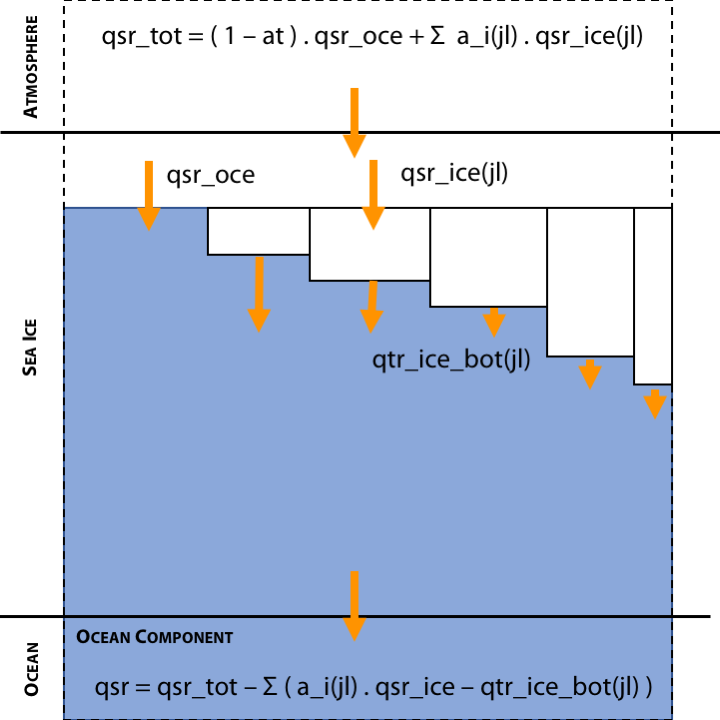
\includegraphics[height=8cm,angle=-00]{../Figures/radiation_atm_ice_oce.png}
\caption{Framing solar radiation transfer through sea ice into the atmosphere-ice-ocean context.}
% ocean uses 0.06 for overcast sky (Payne 74) and Briegleb and Ramanathan parameterization
\label{fig_radiative_transfer}
\end{center}
\end{figure}
%
%--------------------------------------------------------------------------------------------------------------------

\subsection{Forced mode}

In forced-atmosphere mode, it is the incoming solar irradiance fluxes above the ocean and sea ice (categories) that are specified (from files) or computed (from bulk formulae), and constitute the basis of solar radiation transfer computations. Then the net solar fluxes above open water (qsr\_oce) and ice categories (qsr\_ice) are obtained by multiplication by $1-\alpha$. qsr\_tot is then diagnosed as a weighted sum of qsr\_oce and the qsr\_ice(jl)'s.

\subsection{Coupled mode}

In coupled-atmosphere mode, qsr\_tot and qsr\_ice have to be provided by the atmospheric model, whereas qsr\_oce is diagnosed from qsr\_ice and qsr\_tot.

Some atmospheric models enable \textit{tiling} and can provide solar fluxes over individual ice categories. For such atmospheric models, net solar radiation fluxes are directly useable by SI$^3$ (nn\_flxdist =  -1). Other models cannot do tiling, being only able to provide a net solar flux above all ice categories, seen as a single surface type. For such models a first option is to give the net solar flux above sea ice identically to all sea ice categories (nn\_flxdist = 0). Yet a better option is to redistribute the mean solar flux above sea ice $< qsr_ice >$ above categories (nn\_flxdist = 2) using the following scaling, conserving heat by construction:

\begin{eqnarray}
qsr\_ice(jl) = < qsr\_ice > \frac{1 - \alpha(jl)}{1 - < \alpha >}
\end{eqnarray}

where $ < \alpha >$ is the albedo averaged over the ice categories. Note that for testing, the flux redistributor can be emulated in forced mode (nn\_flxdist = 1).

\end{document}